\section{Active Object}

The Active Object design pattern decouples method execution from method invocation to enhance concurrency and simplify synchronized access to objects that reside in their own threads of control.


\subsection{Problem}


Ein Objekt wird von mehreren Threads/Processes benutzt, dabei soll aber eine blockierende Operation nicht alle anderen Clients blockieren.

\subsection{Lösung}


Clients rufen Methoden des Objekts via Proxy auf. Die Proxy wandelt die Aufrufen in MethodRequest's um welche in eine Queue eingefügt werden welche dann von einem Scheduler abgearbeitet wird.
Der Rückgabewert wird via Future-Objekt zurückgegeben.

\subsection{Struktur}


\subsubsection*{Klassendiagramm}

\begin{figure}[H]
	\centering
	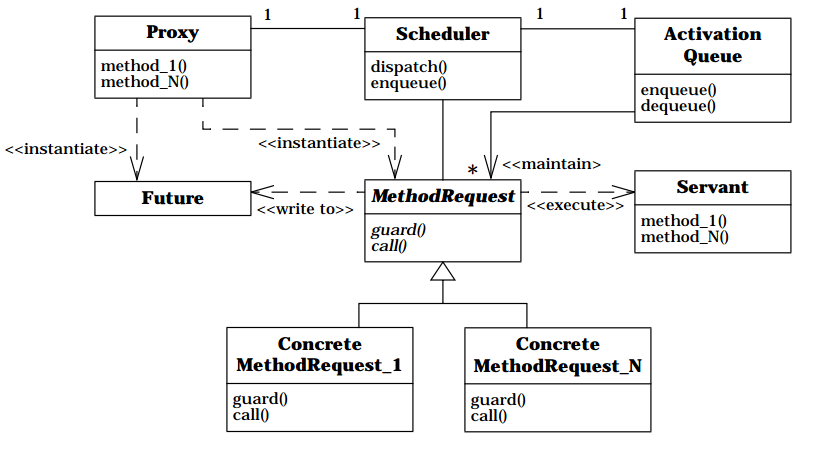
\includegraphics[width=\textwidth]{content/posa2/active-object/images/act-obj_class-diagram.png}
	\caption{act obj class diagram}
\end{figure}


\subsubsection*{Sequenzdiagramm}

\begin{figure}[H]
	\centering
	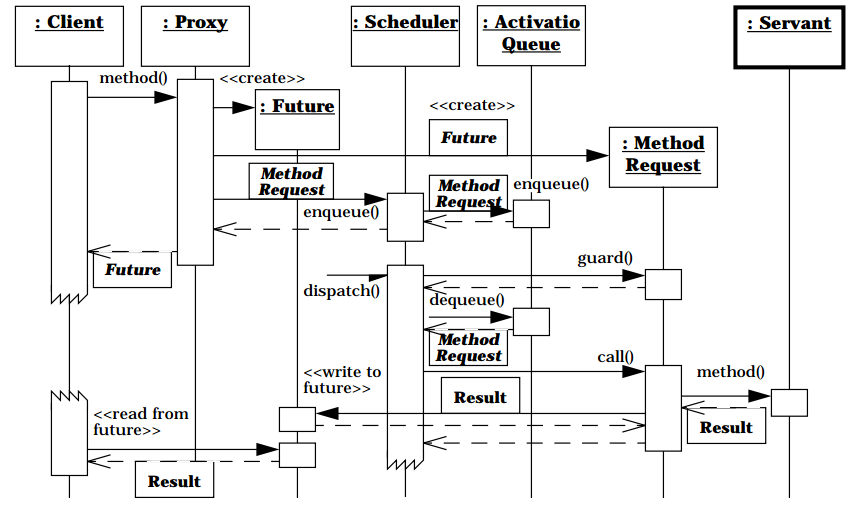
\includegraphics[width=\textwidth]{content/posa2/active-object/images/act-obj_sequence-diagram.png}
	\caption{act obj sequence diagram}
\end{figure}




\subsection{Vorteile}


\begin{itemize}
	\item Methodenaufrufe können zum Client transparent parallelisiert werden
	\item ActiveObject und Proxy können z.B. auch via Netzwerk gekoppelt werden.
\end{itemize}

\subsection{Nachteile}


\begin{itemize}
	\item Erhöhte Komplexität und Implementationsaufwand
	\item Potentieller Performanzverlust
\end{itemize}

\subsection{Known Uses}


\subsection{Prüfungsfragen}


